%!TEX TS-program = xelatex
\documentclass[]{friggeri-cv}
\usepackage{afterpage}
\usepackage{hyperref}
\usepackage{color}
\usepackage{xcolor}
\usepackage{xeCJK}
\usepackage{tikz} 
\usepackage{xcolor}
\usepackage{silence}
\usetikzlibrary{decorations.text}
\usetikzlibrary{shapes}
\setmainfont{Athelas}
\setCJKmainfont[BoldFont={Heiti SC Medium}]{Heiti SC}
\setCJKmonofont{Songti SC}
\setCJKsansfont{Heiti SC}
 \newCJKfontfamily[cuhei]\cuti{Heiti SC Medium}
\hypersetup{
    pdftitle={},
    pdfauthor={},
    pdfsubject={},
    pdfkeywords={},
    colorlinks=false,       % no lik border color
   allbordercolors=white    % white border color for all
}
\addbibresource{bibliography.bib}
\RequirePackage{xcolor}
\definecolor{pblue}{HTML}{0395DE}

\WarningsOff*

\usepackage{enumitem}
\renewenvironment{entrylist}{%
  \begin{itemize}[leftmargin=1in]%[leftmargin=*,align=left,itemindent=-\dimexpr\labelwidth+\labelindent+\labelsep\relax]
}{%
  \end{itemize}
}
\renewcommand{\bfseries}{\headingfont\color{headercolor}}
\renewcommand{\entry}[4]{%
  \item[#1]
    \textbf{#2}%
    \hfill%
    {\footnotesize\addfontfeature{Color=lightgray} #3}\\%
    #4\vspace{\parsep}%
}

\renewcommand{\smallentry}[3]{%
  \item[#1]
    \textbf{#2}%
    \hfill%
    {\footnotesize\addfontfeature{Color=lightgray} #3}\\%
}


\begin{document}
\header{陈载春}{}
      {}
      
% Fake text to add separator      
\fcolorbox{white}{gray}{\parbox{\dimexpr\textwidth-2\fboxsep-2\fboxrule}{%
.....
}}

% In the aside, each new line forces a line break
\begin{aside}
  \section{\cuti 地址}
    重庆市沙坪坝区
    \section{\cuti 生日}
    1985-01
    \section{\cuti 性别}
    男
  \section{\cuti 电话~ QQ~ 微信}
    +86 136 3789 4552
    160 152 79
    czc112358
  \section{Mail}
    \href{mailto:chenzaichun@gmail.com}{\textbf{chenzaichun@}\\gmail.com}
  \section{Web \& Git}
    \href{http://yesokay.herokuapp.com}{yesokay.herokuapp.com}
    \href{https://github.com/chenzaichun}{github.com/chenzaichun}
  \section{\cuti 编程技能}
  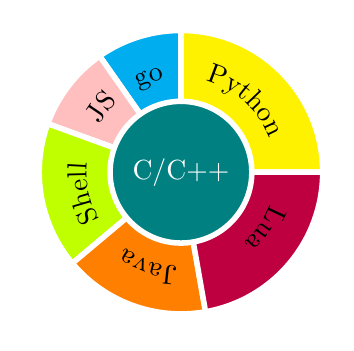
\begin{tikzpicture}[scale=0.6]
\fill [fill=yellow,draw=white,line width=2pt] (0,0) -- (0:3)  arc (0:90:3) -- (0,0);
\draw [decorate,decoration={text along path, text={Python}}] (75:2) arc (75:0:2);
\fill[fill=cyan,draw=white,line width=2pt] (0,0) -- (90:3)  arc [start angle=90, end angle=125, radius=3] -- (0,0);
\draw [decorate,decoration={text along path, text={go}}] (117:2) arc (117:0:2);
\fill[fill=pink,draw=white,line width=2pt] (0,0) -- (125:3)  arc [start angle=125, end angle=160, radius=3] -- (0,0);
\draw [decorate,decoration={text along path, text={JS}}] (150:2) arc (150:0:2);
\fill[fill=lime,draw=white,line width=2pt] (0,0) -- (160:3)  arc [start angle=160, end angle=220, radius=3] -- (0,0);

\draw [decorate,decoration={text along path, text={Shell}}] (210:2) arc (210:0:2);

\fill[fill=orange,draw=white,line width=2pt] (0,0) -- (220:3)  arc [start angle=220, end angle=280, radius=3] -- (0,0);

\draw [decorate,decoration={text along path, text={Java}}] (268:2) arc (268:0:2);
\fill[fill=purple,draw=white,line width=2pt] (0,0) -- (280:3)  arc [start angle=280, end angle=360, radius=3] -- (0,0);
\draw [decorate,decoration={text along path, text={Lua}}] (340:2) arc (340:0:2);
\filldraw[fill=teal,draw=white,line width=2pt] (0,0) circle [radius=3*0.5];
\zihao{0}
\draw (0,0) node[white] {C/C++};
\end{tikzpicture}

  \section{\cuti 操作系统运维}
    \textbf{GNU/Linux}\includegraphics[scale=0.16]{img/5stars}
    \textbf{MacOS}\includegraphics[scale=0.16]{img/4stars}
    \textbf{Windows}\includegraphics[scale=0.16]{img/4stars}
    \textbf{Android}\includegraphics[scale=0.16]{img/3stars}
    \textbf{iOS}\includegraphics[scale=0.16]{img/3stars}
    \textbf{HPUX}\includegraphics[scale=0.16]{img/2stars}
    \textbf{Solaris}\includegraphics[scale=0.16]{img/2stars}
  \section{\cuti 其他技能}
    ~
  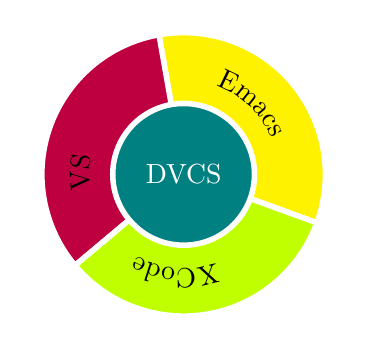
\begin{tikzpicture}[scale=0.6]

\fill [fill=yellow,draw=white,line width=2pt] (0,0) -- (-20:3)  arc (-20:100:3) -- (0,0);
\draw [decorate,decoration={text along path, text={Emacs}}] (70:2) arc (70:0:2);
\fill[fill=purple,draw=white,line width=2pt] (0,0) -- (100:3)  arc [start angle=100, end angle=220, radius=3] -- (0,0);
\draw [decorate,decoration={text along path, text={VS}}] (190:2) arc (190:0:2);
\fill[fill=lime,draw=white,line width=2pt] (0,0) -- (220:3)  arc [start angle=220, end angle=340, radius=3] -- (0,0);
\draw [decorate,decoration={text along path, text={XCode}}] (290:2) arc (290:0:2);
\filldraw[fill=teal,draw=white,line width=2pt] (0,0) circle [radius=3*0.5];
\zihao{1}
\draw (0,0) node[white] {DVCS};

\end{tikzpicture}

    ~
  \section{\cuti 语言}
    \textbf{English}\includegraphics[scale=0.16]{img/3stars}
\end{aside}

\section{\cuti 高等教育经历}
\begin{entrylist}
  \entry
    {2002 - 2006}
    {\cuti 软件工程 学士学位}
    {重庆大学}
    {\\}
  \\}
\end{entrylist}

\section{\cuti 工作经历}
\begin{entrylist}
   \smallentry
  {2017.9 - 至今}
      {云星数据(深圳)有限公司}
      {系统架构}
   \smallentry
  {2010.10 - 2017.8} 
      {Hewlett Packard (HP/HPE)}
      {程序开发}
   \smallentry
    {2008.12 - 2010.9}{重庆支流科技有限公司}{程序开发}
   \smallentry
   {2008.1 - 2008.10}{重庆宏信软件有限责任公司}{程序开发}
   \smallentry
       {2006.7 - 2007.12}{深圳桑德科技有限公司}{程序开发}
\end{entrylist}

\section{\cuti 重要项目经历}
\begin{entrylist}
   \entry
    {2017.9 - 至今}
    {\cuti RightCloud}
    {云星数据}
    {
      RightCloud混合云管理, 让企业摆脱单一云技术带来的束缚和风险,多云异构的混合云管理让选择权回到客户手中,并享受跨云:弹性伸缩、自服务、自动化、综合成本分析等云计算的优势,支持阿里云,华为云,腾讯云,AWS,VMWare,OpenStack,PowerVC,Azure,EasyStack,物理机。
      \newline{\\}
      主要工作是RightCloud产品的设计集成开发,DevOps流水线平台的设计/搭建/开发/维护,Ansible自动化服务编排后台服务的实现, rightcloud agent监控组件的实现, 使用cobbler和MaSS对物理机的管理, CentOS离线Repo的管理,Docker镜像管理与优化, Jenkins Pipeline 实现, 各种POC环境的快速部署, kubernetes环境, All in One快速部署设计实现, IBM power7/8 LPAR的云管设计实现。
      \newline{\\}
      主要客户:海尔,新东方,甘肃万维,东方国信,渤海银行,航天科工,新德汇。
      \\
  技术相关:
  \begin{itemize}
  \item OS: Linux, Unix
  \item 开发工具: Python, go, git, docker, Jenkins, sonarqube, kubernetes
  \end{itemize}
\\}

  \entry
    {2011.4 - 2017.8}
    {\cuti TeMIP Trouble Ticket Liaison}
    {HP}
    {项目主要是给电信厂商提供设备告警和 Trouble Ticket 的管理,并和其他 ITSM 系统集成。
      \newline{\\}
  主要工作是产品的集成开发维护,包括需求分析,升级,设计,开发,实施,支持, patch发布。在该项目中,由于代码历史遗留问题(20+年),程序在不同平台和生产环境上会出现各种崩溃问题。在加入项目后不久,通过对代码的review和优化,程序从原来每周至少有3个不同客户环境的崩溃,到近年来几乎没有任何崩溃。
  \newline
  同时我还参与了很多TeMIP Access Module的开发,包括SNMP, GAT, Corba AM的开发,在开发的过程中,提供了很多小工具用于提高团队的工作效率。
  \\\\
  技术相关:%
  \begin{itemize}%
  \item OS: HP-UX, Linux, Sun Solaris, Windows
  \item 开发工具: C++, shell, gdb, Oracle, Corba, SQL Server, TCP, SVN, VTP, WebService, Java, SNMP
  \end{itemize}
  \\}


    \entry
    {2014.11 - 2015.2}
    {\cuti Vision Media Management}
    {HP}
    {
      Vision Media Management(美国一家电影道具管理和租赁公司)iOS app。我在项目中负责该公司iOS app(该App主要是提供给他们的销售人员用来展示电影中所使用的道具)从iOS6到iOS8的升级。由于在项目中的出色表现,得到客户和项目经理的高度表扬。并协助项目经理完成迪斯尼Game SDK的需求分析。
  \newline{}\newline{}
  技术相关:
  \begin{itemize}
  \item OS: iOS, Mac OSX
  \item 开发工具: Obj-C, XCode, git
  \end{itemize}
\\}

    \entry
    {2010.10 - 2011.4}
    {\cuti GTS V2}
    {HP}
    {该项目主要是给美国通用提供⻋辆自动化测试的工具。负责从V1到V2的升级测试。 收集新需求并发布新版本。 \newline{\\}
      负责从V1到V2的升级测试。
      \newline{}\newline{}
      技术相关:
      \begin{itemize}
      \item OS: Windows
      \item 开发工具: C++ (MFC), Visual Studio, StarTeam
      \end{itemize}
      \\}

    
    \entry
    {2008.12 - 2010.9}
    {\cuti 东方 Online}
    {}
    {3D 武侠⻛格 MMORPG \newline{}
      主要负责服务器端和客户端的开发。包括GUI,背包系统,技能系统等等。
      \newline{}\newline{}
      技术相关:
      \begin{itemize}
      \item OS: Windows
      \item 开发工具: C++, Python, Torque 3D引擎, Excel
      \end{itemize}
      \\}

    \end{entrylist}
    \begin{entrylist}

    \entry
    {2008.1 - 2008.10}
    {\cuti 星球计划}
    {宏信}
    {3D 科幻⻛格 MMORPG, \newline{}
      主要负责客户端逻辑和UI的开发。包括战斗系统,GUI。
      \newline{}\newline{}
      技术相关:
      \begin{itemize}
      \item OS: Windows
      \item 开发工具: C++, Python, Torque 3D引擎, Excel
      \end{itemize}
      \\}

    \entry
    {2006.7 - 2007.12}
    {\cuti 桑德智能⻋载系统}
    {桑德}
    {由深圳桑德电子技术有限公司与重庆大学合作成立重庆大学桑德车载智能化嵌入式实验室,项目首期主要任务是车载智能化平台软件的开发,包括主动安全,移动办公,GPS(第二期),影音媒体等。\newline{}
  在整个项目中(第一期),我的工作是完成倒车雷达(主动安全),蓝牙电话、邮件客户端(移动办公),系统设置,TCPMP移植(媒体播放)等模块及其基础模块的开发。
  \newline{}\newline{}
  技术相关:
  \begin{itemize}
  \item OS: WinCE
  \item 开发工具: C++, Embeded Visual Studio
  \end{itemize}
  \\}

\end{entrylist}


\section{\cuti 证书}
\begin{entrylist}

  \entry
  {\\}
      {ITIL Foundation}
      {\\}
      {\\}
      \\}
\end{entrylist}

\vspace{20pt}

\begin{flushright}
\emph{二〇一九年四月一日}
\end{flushright}
\begin{flushright}
\emph{陈载春}
\end{flushright}

%%% This piece of code has been commented by Karol Kozioł due to biblatex errors. 
% 
%\printbibsection{article}{article in peer-reviewed journal}
%\begin{refsection}
%  \nocite{*}
%  \printbibliography[sorting=chronological, type=inproceedings, title={international peer-reviewed conferences/proceedings}, notkeyword={france}, heading=subbibliography]
%\end{refsection}
%\begin{refsection}
%  \nocite{*}
%  \printbibliography[sorting=chronological, type=inproceedings, title={local peer-reviewed conferences/proceedings}, keyword={france}, heading=subbibliography]
%\end{refsection}
%\printbibsection{misc}{other publications}
%\printbibsection{report}{research reports}

\end{document}
